\documentclass[DIV=calc, paper=a4, fontsize=11pt, twocolumn]{scrartcl}
\usepackage[titletoc,toc]{appendix}
\usepackage[french]{babel}
\usepackage[utf8]{inputenc}
\usepackage[T1]{fontenc}
\usepackage{hyperref}

\hypersetup{
    colorlinks,
    linkcolor={red!50!black},
    citecolor={blue!50!black},
    urlcolor={blue!80!black}
}
\usepackage{amssymb}
\usepackage{graphicx}
\usepackage[protrusion=true,expansion=true]{microtype} 
\usepackage{amsmath,amsfonts,amsthm} 
\usepackage[svgnames]{xcolor} 
\usepackage[hang, small,labelfont=bf,up,textfont=it,up]{caption} 
\usepackage{fix-cm}	 % Custom font sizes - used for the initial letter in the document
\usepackage{subcaption}
\usepackage{sectsty} 
\allsectionsfont{\usefont{OT1}{phv}{b}{n}} 
\usepackage{fancyhdr} 
\pagestyle{fancy} 
\usepackage{lastpage} 

\lhead{}
\chead{}
\rhead{}

% Footers
\lfoot{}
\cfoot{}
\rfoot{\footnotesize Page \thepage\ of \pageref{LastPage}} % "Page 1 of 2"

\renewcommand{\headrulewidth}{0.0pt}
\renewcommand{\footrulewidth}{0.4pt}

\usepackage{lettrine} 
\newcommand{\initial}[1]{ 
\lettrine[lines=3,lhang=0.3,nindent=0em]{
\color{DarkGoldenrod}
{\textsf{#1}}}{}}

\usepackage{titling} % Allows custom title configuration

\newcommand{\HorRule}{\color{DarkGoldenrod} \rule{\linewidth}{1pt}} 

\pretitle{\vspace{-30pt} \begin{flushleft} \HorRule \fontsize{40}{40} \usefont{OT1}{phv}{b}{n} \color{DarkRed} \selectfont} % Horizontal rule before the title

\title{L'Apprentissage Statistique dans L'Analyse Financière des PME} 

\posttitle{\par\end{flushleft}\vskip 0.5em} % Whitespace under the title

\preauthor{\begin{flushleft}\large \lineskip 0.5em \usefont{OT1}{phv}{b}{sl} \color{DarkRed}} % Author font configuration

\author{Juan Barragan} 

\postauthor{\footnotesize \usefont{OT1}{phv}{m}{sl} \color{Black} % Configuration for the institution name

Kommets.com % Your institution

\par\end{flushleft}\HorRule} % Horizontal rule after the title

\date{} % Add a date here if you would like one to appear underneath the title block

%----------------------------------------------------------------------------------------

\begin{document}
\maketitle 
\tableofcontents
\thispagestyle{fancy}
\selectlanguage{french} 
\begin{abstract}
\section{Introduction}
D'après la Fédération des Banques Françaises l'encours de crédits aux PME sur un an (juillet 2015 - juillet 2016) s'élève à 385,2 milliards 
d'euros, ce qui sert à financer plus d'un million d'entreprises. La loi Macron votée en août 2015, permet aux particuliers de financer les PME.
 Dans cette note nous nous proposons de montrer un modèle de Scoring de risque pour les PME basé exclusivement sur leur bilan. 

Nous utiliserons des techniques  dites "big data", notamment \emph{L'Apprentissage Statistique}, pour séparer les indicateurs financiers pertinents et mesurer leur importance dans  la prédiction des faillites. Ceci peux permettre aux particuliers intéressés dans le financement des PME d'en avoir une mesure du risque encouru et donc du niveau attendu de rémunération. 

Nous pensons que le modèle que nous allons prédenter plus un véhicule de mise en relation des investisseurs et entrepreneurs, tel un site internet, permettra de fluidifier le financement, de rémunérer d'avantage les épargnants et soutenir de manière durable l'économie.
\end{abstract}
%----------------------------------------------------------------------------------------
%	ARTICLE CONTENTS
%----------------------------------------------------------------------------------------

\section{Présentation de la base de données d'étude}
La Banque Centrale Française dispose de une base de données des bilans des entreprises mais cette base n'est pas librement disponible. Elle n'est accessible qu'aux établissement de crédit dotés d'un agrément. Il y a la décision du gouvernement à travers les initiatives dites Open Data, de mettre à la disposition du publique les données des entreprises via info-greffe et l'inpi. Mais à l'heure actuelle, ces données ne disposent pas de la granularité que l'on cherche. Pour nos objectifs, la matière brute elle est bien plus importante car elle nous permets d'exploiter librement des indicateurs non concentrés. Les agrégats ayant, souvent, déjà consommé l'information que nous souhaitons exploiter.

Nous avons donc procédé par explorer quelles bases étaient disponibles. Nous n'avons pas trouvé des bases fiables avec matière brute en France. Nôtre choix donc s'est finalement porté sur la Belgique. La banque Centrale Belge (à travers sa \href{https://www.nbb.be/fr/centrale-des-bilans}{Centrale des Bilans}) met à la disposition du publique une base de données complète des bilans des entreprises, avec des historiques portant sur plusieurs décennies. Une participation symbolique nous a permis de disposer d'une édition des bilans des entreprises non consolidés portant sur trois exercices, les années 2013, 2014 et 2015. Aux plus de 350 000 entreprises recensés dans la base nous avons appliqué plusieurs filtres.

\subsection{Les situations juridiques des entreprises}
Parmi la totalité des entreprises nous avons sélectionné celles dont la forme juridique est appropriée pour une étude financière, à savoir:
\begin{itemize}
    \item Société coopérative européenne
    \item Société coopérative à responsabilité illimitée
    \item Société coopérative à responsabilité limitée
    \item Coopérative à responsabilité limitée, coopérative de participation
    \item Société privée à responsabilité limitée
    \item Société en nom collectif
    \item Société en commandite simple
    \item Société en commandite par actions
    \item Société anonyme
    \item Société privée à responsabilité limitée
    \item Société d'assurance mutuelle de droit privé
    \item Société agricole
    \item Société Européenne
    \item Groupement d'intérêt économique avec un siège en Belgique
    \item Groupement européen d'intérêt économique avec un siège en Belgique
\end{itemize}
À ces conditions on ajoute des filtres additionnels concernant le type de faillite pour celles en cessation de payements. Soit l'entreprise est dans une situation juridique normale, soit elle est en
\begin{itemize}
    \item Faillite (ouverture)
    \item Clôture de faillite en cas d'excusabilité
    \item Clôture de faillite sans excusabilité du faillite
\end{itemize}
Ceci nous permet d'analyser les entreprises saines et celles dont un réel défaut est la cause de leur disparition. On évite donc les disparitions dues aux fussions, dissolution anticipées, scissions, etc.  

\subsection{Définition des PME}
Nous souhaitons nous concentrer sur un échantillon d'entreprises, les PME, Petites et Moyennes Entreprises. Selon l'INSEE, la taille répond aux conditions suivantes:
\begin{itemize}
    \item Entreprises occupant moins de 250 employés et dont
    \item Le chiffre d'affaires annuel est inférieur à 50 millions d'euros ou bien un bilan total n'excédant pas les $40$ millions d'euros. Pour éviter les toutes petites entreprises, souvent trop fragiles, 
    \item On exclut les entreprises dont le nombre d'employés est inférieur à 40.
\end{itemize}

\section{Outils}
Pour la réalisation de cette étude, nous avons utilisé des techniques d'apprentissage statistique (Machine Learning), des outils logiciels tels \href{https://www.python.org/}{python} et \href{http://scikit-learn.org/stable/}{scikit} ainsi que des infrastructures permettant le calcul en parallèle \href{http://spark.apache.org/}{Spark}. Les données n'étant pas structurées ni figées ni en nombre constant, notre choix de stockage s'est porté sur la base de données NoSQL \href{https://www.mongodb.com/}{mongo}.

L'apprentissage statistique voit ses origines dans l'ingénierie et la science informatique. C'est une branche de la science utilisant 
des méthodes statistiques pour déceler des patrons. 

Nous nous intéressons à ces méthodes car nous allons explorer plusieurs millions de données comptables à la recherche d'un patron permettant de savoir lorsque une entreprise, au vue de leurs bilans, est proche d'une cessation de payements. 

C'est une étude habituellement réalisée par des analystes financiers d'une manière plutôt manuelle et avec des critères empiriques pour repérer des seuils critiques. Notre propos ici c'est de formaliser ces méthodologies et de trouver de manière précise ces seuils.

\subsection{Analyse par composantes principales}
\emph{L'analyse par Composantes Principales} est une méthodologie Statistique permettant de convertir une suite de vecteurs $X_1, X_2, \ldots X_k$, $X_i \in \mathbb{R}^n$ dans un ensemble de variables $Y_1, Y_2, \ldots Y_k$ $Y_i \in \mathbb{R}^m$, avec $m \leq n$ qui ne sont pas corrélées. Les vecteurs $Y_i$ sont appelés \emph{Composantes Principales} et le fait que leur dimension puisse être moindre, tout en préservant la variance, est d'une grande utilité lorsque on cherche à visualiser un nombre important d'observations. 

Techniquement on peut calculer ces composantes de la manière suivante, soit $\mathbf{m}$ le vecteur moyen, $\mathbf{m} = \sum_{i=1}^k X_i$, soit $\mathbf{S}$ la matrice de covariance $\mathbf{S} = 1/k \sum_{i=1}^k (X_i - \mathbf{m})(X_i - \mathbf{m})^t$, $X^t$ étant le vecteur transposé de $X$. Pour réduire sur un espace $m$ dimensionnel il suffit de calculer les $m$ vecteurs propres de $\mathbf{S}$ $v_1, \ldots v_m$, possédant les plus grands valeurs propres. On forme une matrice de dimension $n \times m$, $\mathbf{W} = (v_1, \ldots v_m)$. L'espace $Y$, que l'on cherche est donné par $Y = \mathbf{W}^t X$.
\subsection{K-Moyennes, algorithme de Lloyd}
Les $K-$ moyennes sont une méthode pour trouver des agrégats dont les valeurs sont proches dans un ensemble de données ne possédant pas d'étiquettes. Étant donné $m$ valeurs $X_1, X_2, \ldots X_m$ et un entier $k$, on cherche $k$ agrégats dépendant de $k$ centres $c_1, c_2, \ldots c_k$ comme suit:
\begin{itemize}
  \item[0] Choisissons la première itération de centres $c_1^0, c_2^0, \ldots c_k^0$ au hasard mais tous différents.
  \item[1] On définit les agrégats 
    $$S_i^n = \{ X : \| X - c_i^n \| \leq \|X - c_j^n \| \quad \forall i \neq j \}$$
  \item[2] Ensuite les nouveaux centres
    $$c_i^{n+1} = \frac{1}{|S_i|} \sum_{X \in S_i} X$$
avec $|S_i|$ le nombre d'éléments dans $S_i$.
  \item[3] on répète depuis le pas $1$ et $2$ jusqu'à un certain seuil de tolérance.
\end{itemize}
\begin{figure}
  \centering
    
\includegraphics[width=0.5\linewidth]{centers}
  \caption{Agrégats de l'algorithme $K$-Moyennes}
  \label{fig:kmeans}
\end{figure}
Dans la figure \ref{fig:kmeans} on observe un exemple d'agrégat avec 9 bassins.
\subsection{La régression logistique}
Soit à nouveau $X_1, X_2, \ldots X_k$, $X_i \in \mathbb{R}^n$ une suite de points et $\lambda : \mathbb{R}^n \to \{0,1\}$ un système \emph{d'étiquettes}. Soit $Y_i = \lambda(X_i)$ on peut considérer $Y$ comme une variable aléatoire de Bernoulli. Écrivons pour la probabilité, étant donné une valeur $X_0$,
$$\mathbb{P}(Y=1| X = X_0) = p,$$
$$\mathbb{P}(Y=0| X = X_0) = 1-p$$
ou plus compactement:
\begin{equation}
\mathbb{P}(Y=Y_0| X = X_0) = p^{Y_0}(1-p)^{1-Y_0}.
\label{eqn:bern}
\end{equation}
C'est donc un problème de classification, dans l'idéal, il existe un plan $L: \mathbb{R}^n \to \mathbb{R}$, $L_{\theta, \theta_0}(X) = \theta X + \theta_0$ qui sépare les deux étiquettes. C'est à dire tel que
$$ L_{\theta, \theta_0}(X_i) > 0, \quad \text{si} \quad Y_i = 1, \quad \text{et}$$
$$ L_{\theta, \theta_0}(X_i) < 0, \quad \text{si} \quad Y_i = 0.$$
On peut lier le plan séparateur à notre variable de Bernoulli avec la fonction, $s(x) = 1/(1+ e^{-x})$. Il suffit d'écrire pour chaque observation $X_i$, 
\begin{align*}
p &= \mathbb{P}(Y=1|X_i)\\
                    &= \frac{1}{1+ e^{-L_{\theta, \theta_0}(X_i)}}\\
\end{align*}
On peut donc réécrire \ref{eqn:bern} comme
%\begin{align*}
$$\left( \frac{1}{1 + e^{-L_{\theta, \theta_0}(X_i) }} \right)^{Y_i} \left ( 1- \frac{1}{1 + e^{-L_{\theta, \theta_0}(X_i) }} \right)^{1 - Y_i} $$
%\end{align*}
ou bien
$$\frac{e^{-L_{\theta, \theta_0} (X_i)^{1-Y_i}}}{1 + e^{-L_{\theta, \theta_0}(X_i)}}$$
Pour trouver les paramètres optimaux $\theta, \theta_0$ nous maximisons le logarithme de la \emph{vraisemblance} sur la totalité des observations:
$$\textbf{argmax}_{\theta, \theta_0}\log \prod_{i=1}^k \frac{e^{-L_{\theta, \theta_0} (X_i)^{1-Y_i}}}{1 + e^{-L_{\theta, \theta_0}(X_i)}}$$
\begin{figure}
  \centering
    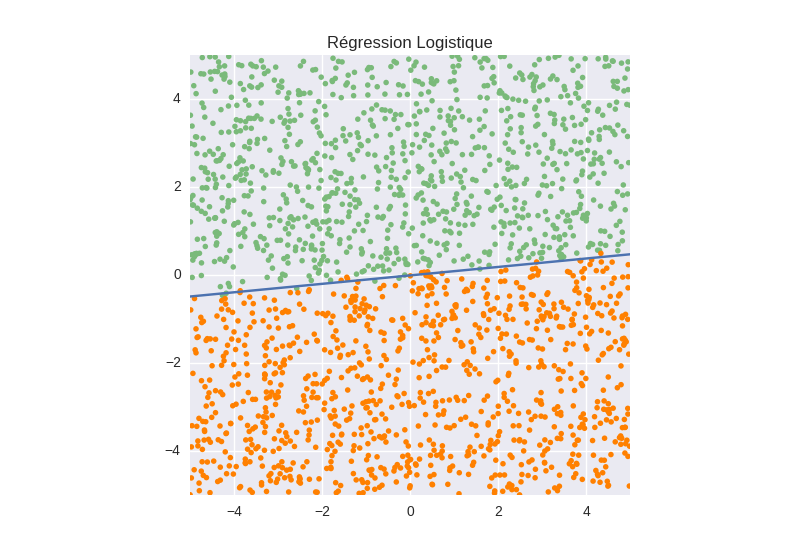
\includegraphics[width=\linewidth]{reglog}
  \caption{Régression Logistique}
  \label{fig:reglog}
\end{figure}
Dans la figure \ref{fig:reglog} un exemple de régression logistique et son plan séparateur.
\subsection{Les Machines à Support Vectoriel (SVM)}
Une méthodologie similaire à la régression logistique est les \emph{machines à support vectoriel}. On se place dans un cadre similaire à la section précédente, avec une suite d'observations $X_1, X_2, \ldots X_k$, $X_i \in \mathbb{R}^n$, mais on change légèrement nos étiquettes $\lambda : \mathbb{R}^n \to \{1, -1\}$. Si un plan séparateur existe, $L: \mathbb{R}^n \to \mathbb{R}$, $L_{\theta, \theta_0}(X) = \theta X + \theta_0$ tel que $\textrm{sign}(L_{\theta, \theta_0}(X_i)) = \lambda(X_i)$. On a pour tout $i$
\begin{equation}
\frac{\lambda_i(X_i)L(X_i)}{\|\theta\|}>0
\label{eqn:dist}
\end{equation}
On reconnais dans la formule \ref{eqn:dist} la distance du point $X_i$ au plan $L_{\theta, \theta_0}$. La machine à support vectoriel c'est la solution qui maximise cette distance:
\begin{equation}
\textbf{argmax}_{\theta, \theta_0} \left\{ \frac{1}{\|\theta\|} \textbf{min}_i\lambda(X_i)L_{\theta, \theta_i}(X_i)\right\}
\label{eqn:svm}
\end{equation}
Pour simplifier le programme de maximisation \ref{eqn:svm} on change l'échelle du plan $\theta \to \kappa \theta$ et $\theta_0 \to \kappa \theta_0$ de sorte que si $X_p$ est le point réalisant le minimum $\textbf{min}_i\lambda(X_i)L_{\theta, \theta_i}(X_i)$, alors pour ce point $X_p$ on a $\lambda(X_p)L_{\theta, \theta_0}(X_p) = 1$. Le programme d'optimisation \ref{eqn:svm} peut donc s'écrire:
$$\textbf{argmax}_{\theta, \theta_0}  \frac{1}{\|\theta\|}, \quad i = 1, \dots k$$
ou de manière équivalente: 
$$\textbf{argmin}_{\theta, \theta_0}  \frac{1}{2}\|\theta\|^2, \quad i = 1, \dots k$$
sous les contraintes
$$ \lambda(X_i)L_{\theta, \theta_0}(X_i) \geq 1 \quad i = 1, \ldots k$$
\begin{figure}
  \centering
    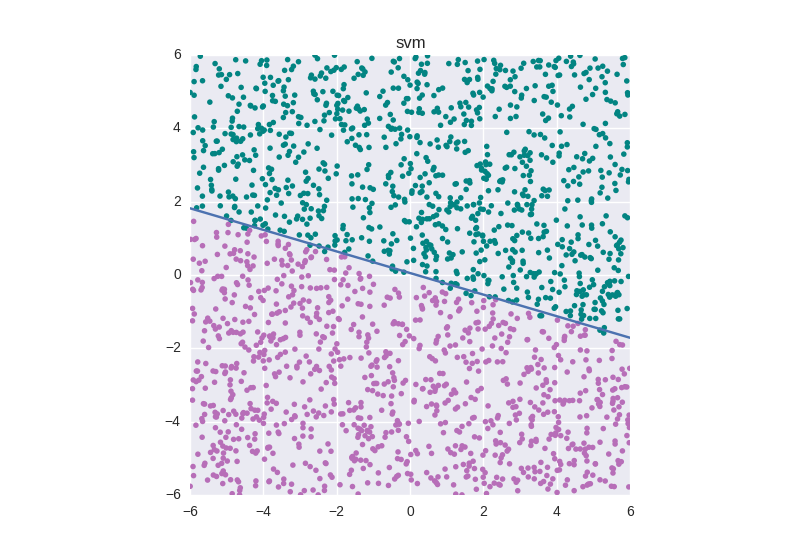
\includegraphics[width=\linewidth]{svm}
  \caption{Engin à Support Vectoriel}
  \label{fig:svm}
\end{figure}
Dans la figure \ref{fig:svm} un exemple d'une machine à support vectoriel et son plan séparateur.

\section{Analyse des Ratios Financiers}
Traditionnellement la solidité d'une entreprise passe par l'analyse financière de ses ratios comptables. Les experts métier utilisent les bilans de l'entreprise pour calculer des quotients qui permettent la visualisation de sa situation économique. 

Les ratios les plus parlants ce sont, \emph{le ratio de marge}, \emph{ratio d'endettement}, \emph{rentabilité de l'actif}, \emph{rentabilité des capitaux employés, ROCE}, \emph{rentabilité financière, ROE}, \emph{résultat opérationnel, EBIT*}. Le lecteur non familiarisé avec ces termes peux consulter \cite{Thibierge} pour les définitions et détails.
\subsection{Le modèle d'Altman}
Nous nous sommes inspirés du modèle de Scoring d'Altman pour détecter les entreprises en difficulté, voir \cite{Altman}. Dans ce modèle, l'auteur propose une analyse de discriminants multiples basés sur des ratios financiers. La fonction discriminante étant un plan $Z = V_1X_1 + V_2X_2 + \ldots V_nX_n$, les $V_i$ étant des coefficients discriminants et $X_i$ les variables indépendantes représentant les ratios financiers issus des bilans des entreprises. Altman établit un score, le niveau duquel étant directement lié à la solidité de l'entreprise.

Notre objectif c'est de généraliser cette fonction discriminante utilisant l'apprentissage statistique. Nous allons notamment utiliser la régression logistique et les machines à support vectoriel pour estimer les coefficients discriminants. 

Dans son étude, Altman trouve une fonction discriminante de la forme
\begin{align*}
Z =& \enskip 0.012X_1  + 0.014X_2 + \\
  & \enskip 0.033X_3 +   0.006X_4 +  0.999X_5\\
\end{align*}
avec les ratios suivants:
\begin{itemize}
  \item[] $X_1$ Les capitaux engagés sur les actifs totaux,
  \item[] $X_2$ Les bénéfices non distribués sur les actifs totaux,
  \item[] $X_3$ L'EBDITA, Revenus avant dépréciations, Intérêts Taxes et Amortisations sur les actifs totaux,
  \item[] $X_4$ La valeur boursière de l'entreprise sur la valeur de la dette,
  \item[] $X_5$ Le total des ventes sur les actifs totaux.
\end{itemize}
Nous aussi, nous allons obtenir également un plan discriminant avec leurs poids permettant de donner un score de risque à chaque entreprise de l'échantillon.

\subsection{Les Ratios la Banque Centrale Belge}
Les ratios que nous allons utiliser son au nombre de $21$ et sont calculés par la Banque Centrale Belge. Nous les présentons de manière sommaire dans l'appendice. 

Nous ne pouvons pas utiliser la méthodologie d'Altman car elle suppose que l'entreprise est cotée en bourse ce qui n'est pas le cas dans la majorité des PME.
Notre échantillon de PME belges, celles dont le bilan total n'excède pas les 40 million d'Euros et ayant au moins 40 employés compte $4796$ entreprises. Parmi ces entreprises 45 ont fait faillite: 22 en 2015, 22 en 2014 et une en 2013.

On aperçois immédiatement une grande difficulté: la rareté des défauts. On a moins de $1\%$. 
Une analyse par composante principales des ratios au $2014$ montre une difficulté additionnelle, voir la figure \ref{fig:pca2D}: les entreprises en défaut sont aussi dispersées. Pour illustrer les inconvénients de l'apprentissage statistique avec ce type de population, nous allons lui appliquer les méthodes de régression logistique et machine à support vectoriel. On se place sur les données 2014 en excluant l'entreprise qui à fait défaut en 2013. Les figures \ref{fig:elog} et \ref{fig:esvm} illustrent les résultats de la régression logistique et de l'engin à support vectoriel projetés sur le plan.
\begin{figure}
  \centering
    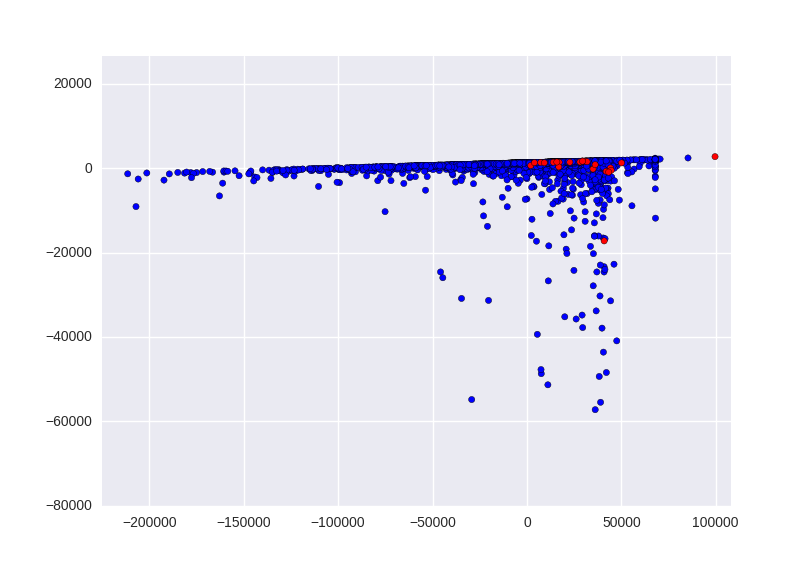
\includegraphics[width=\linewidth]{pca2D}
  \caption{PCA 2D, ratios 2014}
  \label{fig:pca2D}
\end{figure}
\begin{figure}
  \centering
    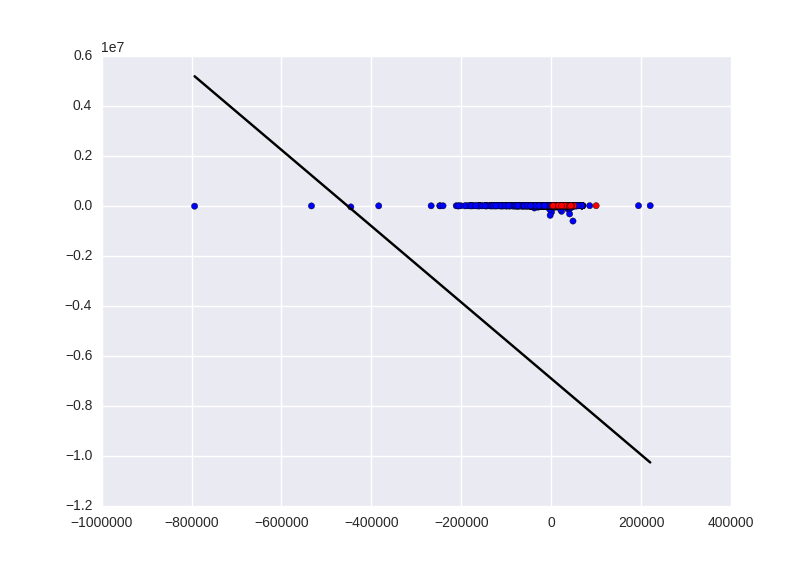
\includegraphics[width=\linewidth]{elog}
  \caption{Régression logistique}
  \label{fig:elog}
\end{figure}
\begin{figure}
  \centering
    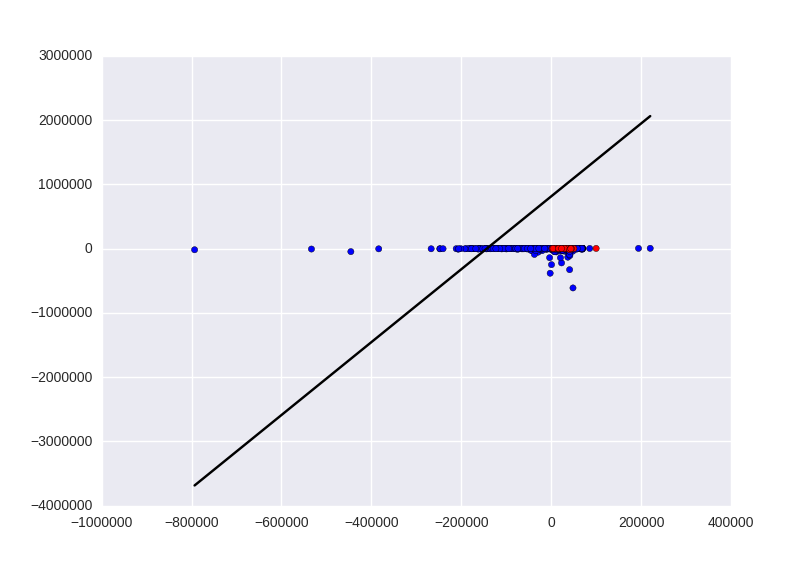
\includegraphics[width=\linewidth]{esvm}
  \caption{Engine à support vectoriel}
  \label{fig:esvm}
\end{figure}

Les résultats sont médiocres, aucune méthode n'arrive à séparer les données. 

\subsection{Sélection d'un échantillon}
Nous souhaitons nous affranchir du problème concernant la rareté des données. Pour ce faire nous nous sommes inspirés de l'article d'Altman qui suggère de construire un échantillon plus petit. 

On prend la totalité des entreprises en défaut mais on fait une sélection sur les entreprises saines.
Soit $\mathcal{E}$ l'ensemble d'entreprises, $\mathcal{S}$ les entreprises saines et $\mathcal{D}$ celles qui sont en faillite. Pour chaque entreprise $e$ il existe sa suite de ratios $r_i(e)$. Soit
$$R_i = \max \{ r_i(e) | e \in \mathcal{D} \},$$
$$E_i = \{ e \in \mathcal{S} : r_i(e) \geq R_i \}$$
On cherche une suite de ratios, $r_i$ tels que $\cap E_i \neq \varnothing$ et dont la cardinalité soit comparable à celle des entreprises en faillite, $\#\cap E_i \sim \#\mathcal{D}$. 

Après un calcul poussé effectué avec \href{http://spark.apache.org/}{Spark} portant sur la totalité des intersections et une analyse minutieux des résultats, nous avons retenu les ratios suivants:
\begin{itemize}
\item marge nette sur ventes
\item valeur ajoutée par personne, 
\item Rentabilité nette des capitaux propres après impôts,
\item Rentabilité nette de l’actif total avant impôts et charges de dettes,
\item Liquidité au sens strict et
\item Capitaux propres / Ensemble des moyens d’action.
\end{itemize}
Nous présentons les graphiques de dispersion en annexe.
Les résultats obtenus, très encourageants, sont présentés dans la figure \ref{fig:reglogsample}. On a réalisé un graphique de contour représentant la probabilité de survie. Le tout projeté sur deux dimensions en composantes principales.
\begin{figure}
  \centering
    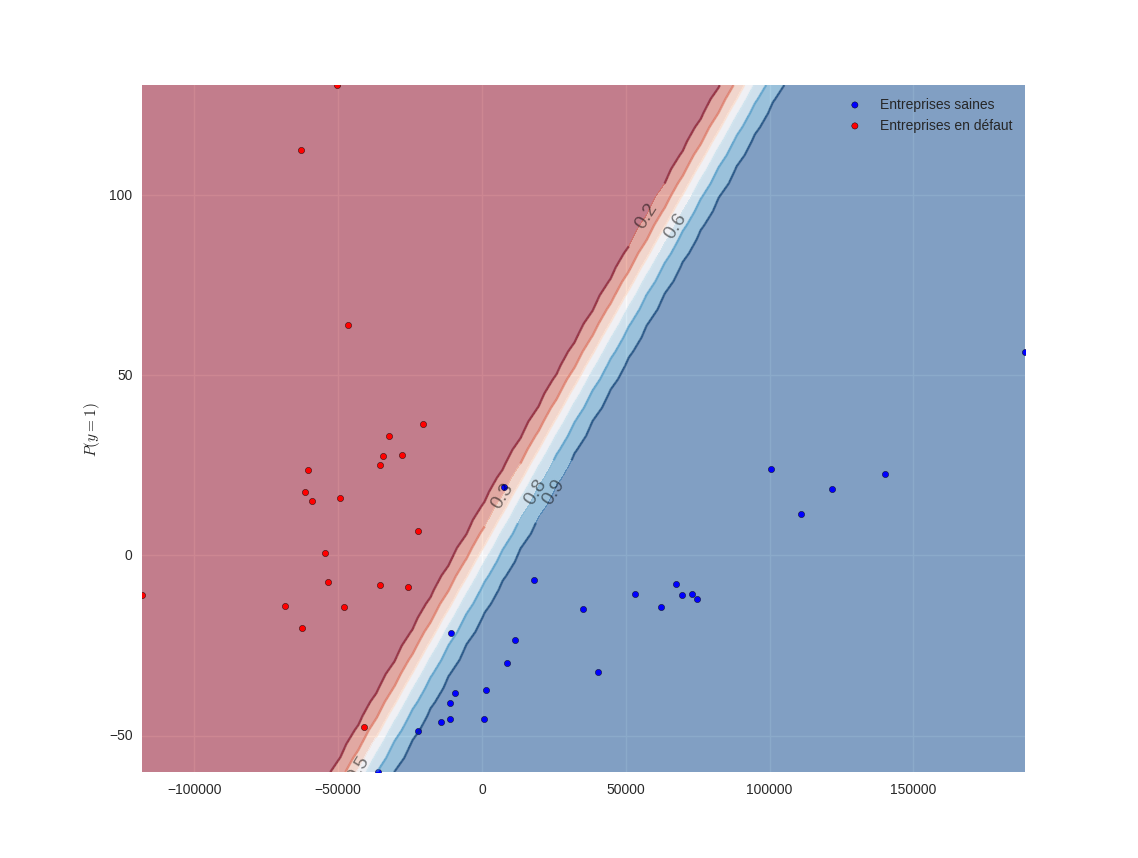
\includegraphics[width=\linewidth]{reglogsample}
  \caption{Régression logistique, probabilité de survie}
  \label{fig:reglogsample}
\end{figure}

\section{Scoring}
Maintenant que nous disposons d'un bon échantillon, nous souhaitons étendre la méthode logistique à l'ensemble des entreprises. Plusieurs métriques concernant la qualité de notre classement nous intéressent. Nous souhaitons exprimer la solidité d'une entreprise utilisant un \emph{score} $R$. Si $\mathbb{P}_t(e|r) = \mathbb{P}_t(e| r_i, i=1, \dots n)$ est la probabilité de survie d'une entreprise à une date future $t$ étant donné ses ratios actuels $r = r_1, \ldots r_n$ . Nous cherchons un score $R$ tel que
$$R(e_1) \leq R(e_2)$$
alors la 
$$\mathbb{P}_t(e_1| r) \leq \mathbb{P}_t(e_2| r)$$
Autrement dit un meilleur score se traduit par une meilleur probabilité de survie.
\subsection{Métriques et erreurs de classification}
Étant donné un classificateur on s'intéresse à sa qualité en mesurant la quantité d'erreurs lors du classement. 

Dans notre cas cette mesure n'est pas pertinente. L'ensemble d'entreprises en défaut ne représente que $0.5\%$ de la population sur une année. Un classificateur classant toute entreprise comme saine ne commettra qu'une erreur de $0.5\%$.  

De ce fait, on s'intéresse plutôt aux \emph{Vrais Positifs} et \emph{Vrais Négatifs} c'est à dire:
\begin{itemize}
\item[] Vrais Positifs (TP), ces entreprises bien classées et étant en bonne santé,
\item[] Vrais Négatifs (TN), ces entreprises classés mauvaises et étant en faillite.
\end{itemize}
La \emph{F-mesure} considère les quotients $TP/S$ et $TN/D$, $S$ étant les entreprises saines et $D$ celles en faillite. Autrement dît le pourcentage d'erreur parmi les bonnes entreprises et le pourcentage d'erreur parmi les entreprises en faillite. Pour un investisseur il est plus important détecter les \emph{Vrais Négatifs}. En effet une erreur Vrai Positif est une opportunité d'investissement perdue, mais une erreur Vrai Négatif est un mauvais investissement. Notre première métrique est une F-Mesure modifiée:
$$ F = \frac{1}{3}\frac{TP}{S} + \frac{2}{3}\frac{TN}{D}$$
Soit $E$, l'ensemble d'entreprises, pour un score donné $R$, on lui associe sa fonction de distribution
$$F_R(x) = \frac{1}{|E|} | \{ e \in E | R(e) \leq x \} | $$
Notre métrique suivante veux que les entreprises en défaut au temps $t$, $D_t$ aient un mauvais score:
$$M_t = 1 - \frac{1}{|D_t|} \sum_{e \in D_t} F_R(e)$$
\subsection{Score naturel}
Notre choix de score se porte naturellement sur le plan séparateur de la régression logistique. 
$$L_{\theta, \theta_0}(X) = \sum_{i=1} \theta_i X_i + \theta_0$$
Ce plan sépare les bonnes entreprises des mauvaises. La distance d'un point $X$ à ce plan étant donné par
$$d(X, L_{\theta, \theta_0}) = \frac{L_{\theta, \theta_0}(X)}{\| \theta \|}$$
Cette distance est donc un bon indicateur de la proximité de l'entreprise vers la zone à risque. 

Si $r_1, \ldots r_n$ sont les ratios de l'entreprise, notre score sera défini par:
$$HS(e) = \sum_{i=1}^n \theta_i r_i$$
avec $\theta = (\theta_1, \ldots, \theta_n)$ les coefficients discriminateurs de la régression logistique.

Nous disposons de 21, certainement il y a des corrélations entre eux. Nous souhaitons réduire le nombre de ratios et calibrer les coefficients. Notre métrique total fait appel à la section précédente, nous allons mesurer la qualité d'un score $R$ par la métrique suivante:
$$\frac{F + M_{2014} + M_{2015}}{3}$$
En mots: un score es préférable si:
\begin{itemize}
\item il est prudent, on est plus concernés par les  mauvais investissements plutôt que aux opportunités ratés.
\item les entreprises en faillite au 2014 sont mal scorées
\item les entreprise en faillite au 2015 sont mal scorées
\end{itemize}
\subsection{Méthodologie}
Nous allons donc éliminer les ratios non pertinents. pour l'accomplir nous allons faire un calcul exhaustif. Nous allons calculer les métriques pour les scores issus des $2^{21} = 2 097 152$ combinaisons possibles. C'est un calcul parallèle que nous avons implémente avec  \href{http://spark.apache.org/}{Spark}.

\subsection{Résultats}
Nos avons sélectionné parmi les meilleures métriques l'ensemble de ratios financièrement plus parlants et en nombre le plus petit. On en recense donc un ensemble de neuf ratios:
\begin{itemize} %r4,r5,r6,r9,r10,r11,r12,r17,r19
  \item $X_1=$ Valeur ajoutée par personne occupée,
  \item $X_2=$ Valeur ajoutée / Immobilisations corporelles brutes,
  \item $X_3=$ frais de personnel / Valeur ajoutée,
  \item $X_4=$ Rentabilité nette des capitaux propres après impôts,
  \item $X_5=$ Cash-flow / Capitaux propres,
  \item $X_6=$ Rentabilité brute de l’actif total avant impôts sur charges des dettes,
  \item $X_7=$ Rentabilité nette de l’actif total avant impôts et charges des dettes, 
  \item $X_8=$ Nombre de jours de crédit clients sur chiffre d'affaires,
  \item $X_9=$ Capitaux propres / Ensemble des moyens d’action.
\end{itemize}
Aprês application d'une régression logistique nous trouvons le score défini par 
\begin{multline}
HS(X) = 0.000085X_1+0.000072X_2-0.064981X_3\\
+0.025403X_4-0.009528X_5+0.010398X_6\\
+0.017364X_7-0.014765X_8+0.018111X_9
\end{multline}
Nous remarquons un résultat intéressant: deux éléments ont un impact négatif sur le score, les frais de personnel sur valeur ajoutée et le nombre de jours de crédit clients. 

La table suivante résume les résultats obtenus:
\begin{center}
  \begin{tabular}{ | r || l |}
    \hline
    Nombre d'entreprises & 4795  \\ \hline
    En faillite 2014 & 22  \\ \hline
    En faillite 2015 & 22  \\ \hline
    Seuil de défaut 2014 & -2.018 \\ \hline
    quantile du seuil 2014 & 25.14\% \\ \hline
    Erreur en 2015 & 9.1\% \\ \hline
  \end{tabular}
\end{center}
Le \emph{seuil de défaut} Veux dire que pour les ratios 2014, toutes les entreprises en faillite sont au dessous. En contrepartie de cela, le quantile de $25.14\%$ veux dire grosso-modo que $24\%$ des bonnes entreprises sont mal classées (Mais c'était un objectif, nôtre classement est conservateur). Seulement deux entreprises (moins de 10\%) parmi les 22 ayant fait défaut en 2015 dépassent ce seuil. C'est un très bon résultat.

Dans un deuxième pas nous souhaiterons étendre ces analyses sur plusieurs années.
\begin{appendices}
\section{Les ratios de la Banque Centrale Belge}
Nous allons énumérer les ratios utilisés. Le lecteur intéressé par une définition précise des ratios, ainsi que leur méthodologie de calcul à partir d'un bilan peut consulter le site de la Banque Centrale Belge, \href{https://www.nbb.be/fr/centrale-des-bilans}{Centrale des Bilans}
\begin{enumerate}
\item Marge brute sur ventes
\item Marge nette sur ventes
\item Taux de valeur ajoutée
\item Valeur ajoutée par personne occupée (en EUR)
\item Valeur ajoutée / Immobilisations corporelles brutes
\item Frais de personnel / Valeur ajoutée
\item Amortissements, réductions de valeur et provisions pour risques et charges / Valeur ajoutée 
\item Charges des dettes / Valeur ajoutée 
\item Rentabilité nette des capitaux propres après impôts
\item Cash-flow / Capitaux propres
\item Rentabilité brute de l’actif total avant impôts
\item Rentabilité nette de l’actif total avant impôts
\item Liquidité au sens large
\item Liquidité au sens strict
\item Rotation des stocks d'approvisionnements et de marchandises
\item Rotation des stocks d'en-cours de fabrication et de produits finis
\item Nombre de jours de crédit clients
\item Nombre de jours de crédit fournisseurs
\item Capitaux propres / Ensemble des moyens d’action
\item Acquisitions d'immobilisations corporelles / Valeur ajoutée
\item Acquisitions d'immobilisations corporelles / Immobilisations corporelles au terme de l'exercice précédent
\end{enumerate}

\onecolumn
\section{Histogrammes des distributions}
Nous étudions l'agrégat des ratios des entreprises pour l'année 2014 en excluant l'entreprise qui a fait défaut en 2013. Un premier aperçu du pouvoir discriminant des ratios est obtenu en réalisant des histogrammes sur la distributions de ratios. Dans l'axe horizontal nous avons illustré en rouge les ratios des entreprises qui sont en faillite.

Dans l'idéal les entreprises en rouge sont concentrées dans une région contenant peu de densité dans l'histogramme. C'est le cas de la figure b), valeur ajoutée par personne. Mis à part une probable aberration statistique la plupart de points rouges sont concentrés sur la partie gauche de l'histogramme.
\begin{figure}[H]
\centering
\captionsetup[subfigure]{labelformat=empty}
  \begin{subfigure}{.45\textwidth}
    \centering
    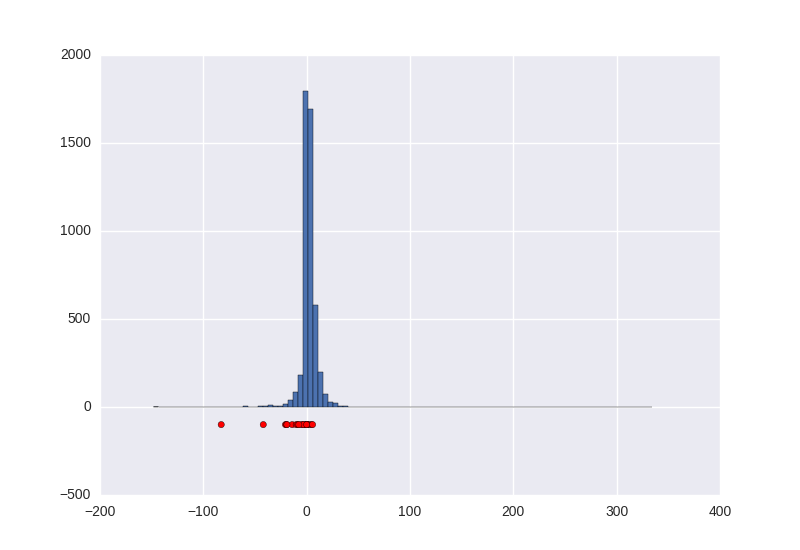
\includegraphics[width=\linewidth]{r2.png}
    \caption{Marge nette sur ventes}
  \end{subfigure}
  \begin{subfigure}{.45\textwidth}
    \centering
    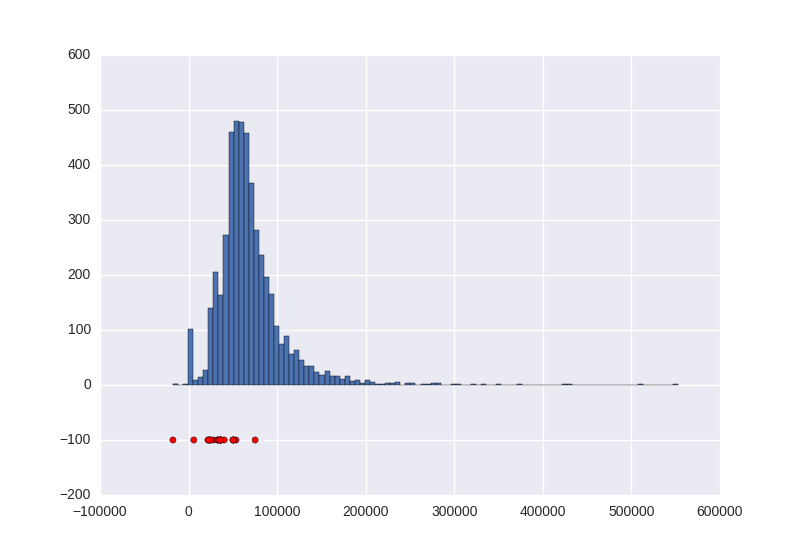
\includegraphics[width=\linewidth]{r4.png}
    \caption{Valeur ajoutée par personne}
  \end{subfigure}
  \begin{subfigure}{.45\textwidth}
    \centering
    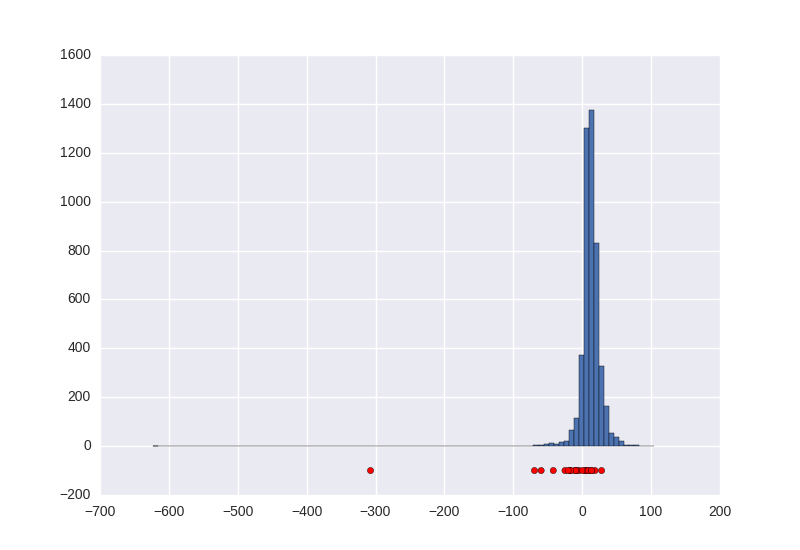
\includegraphics[width=\linewidth]{r11.png}
    \caption{Rentabilité brute de l’actif total avant impôts}
  \end{subfigure}
  \begin{subfigure}{.45\textwidth}
    \centering
    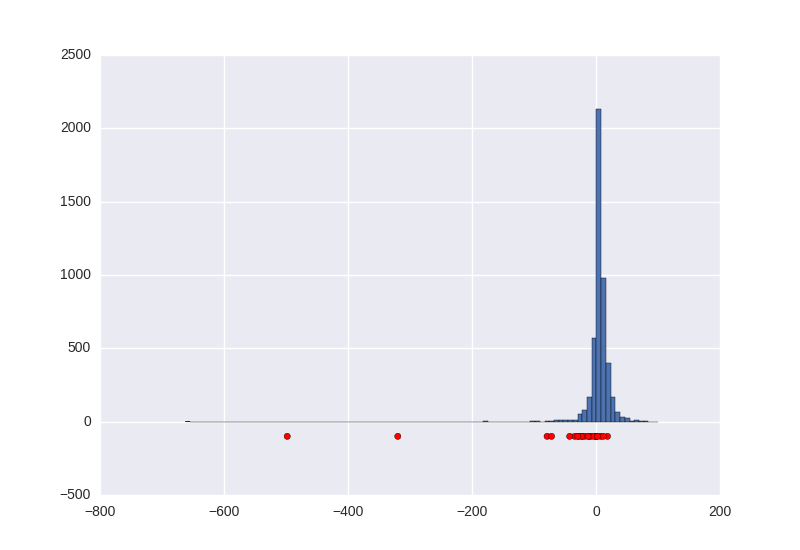
\includegraphics[width=\linewidth]{r12.png}
    \caption{Rentabilité nette de l’actif total avant impôts}
  \end{subfigure}
\caption{Diagrammes de distribution }
\end{figure}

\begin{figure}
\captionsetup[subfigure]{labelformat=empty}
  \begin{subfigure}{.45\textwidth}
    \centering
    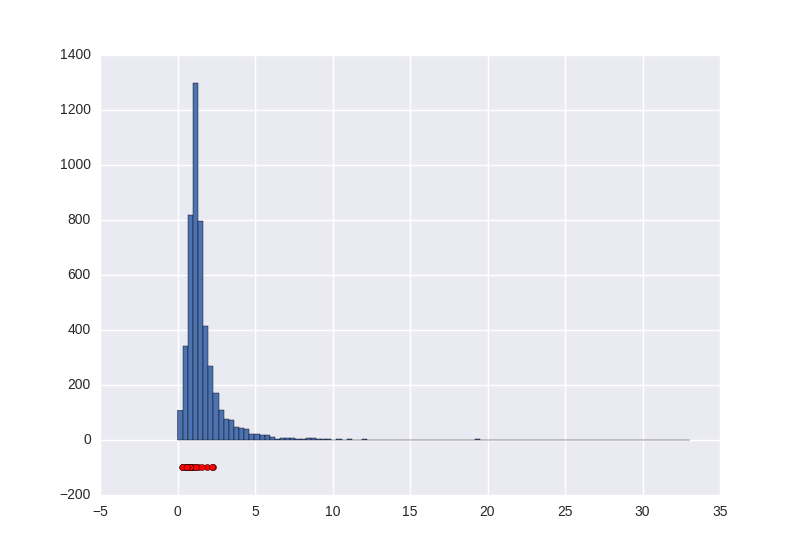
\includegraphics[width=\linewidth]{r13.png}
    \caption{ Liquidité au sens large}
  \end{subfigure}
  \begin{subfigure}{.45\textwidth}
    \centering
    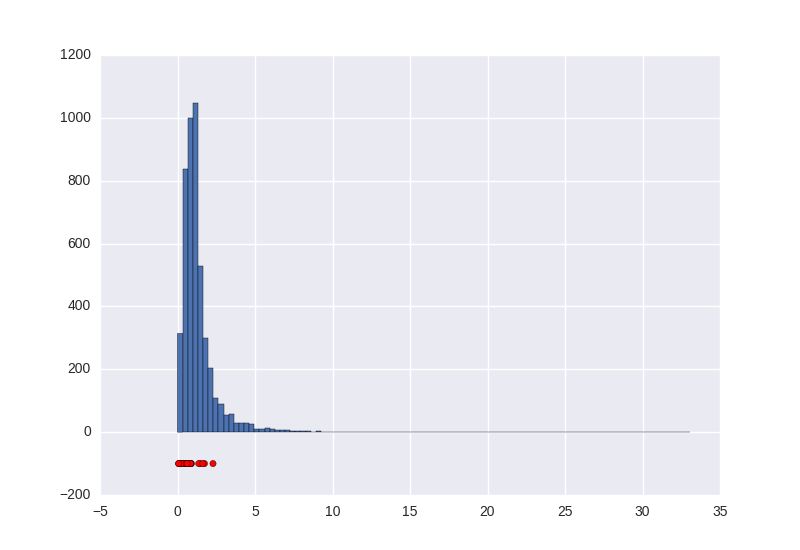
\includegraphics[width=\linewidth]{r14.png}
    \caption{Liquidité au sens strict}
  \end{subfigure}
  \begin{subfigure}{.45\textwidth}
    \centering
    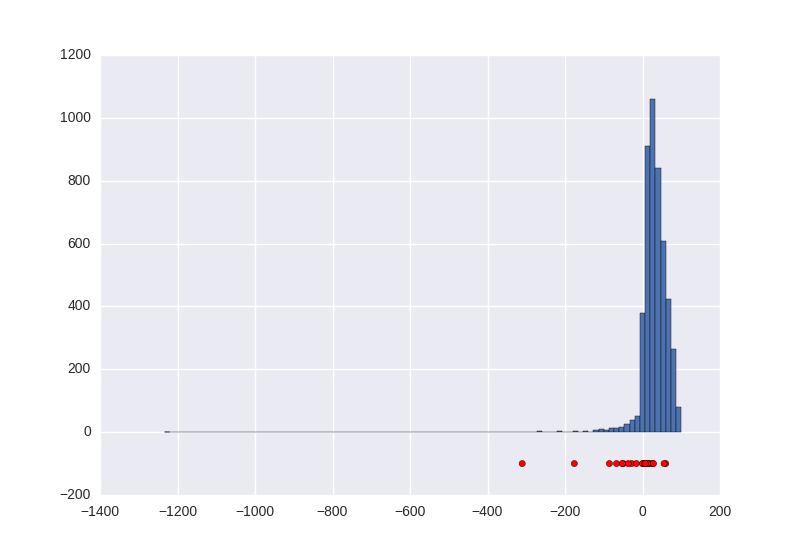
\includegraphics[width=\linewidth]{r19.png}
    \caption{Capitaux propres / Ensemble des moyens d’action}
  \end{subfigure}
  \begin{subfigure}{.45\textwidth}
    \centering
    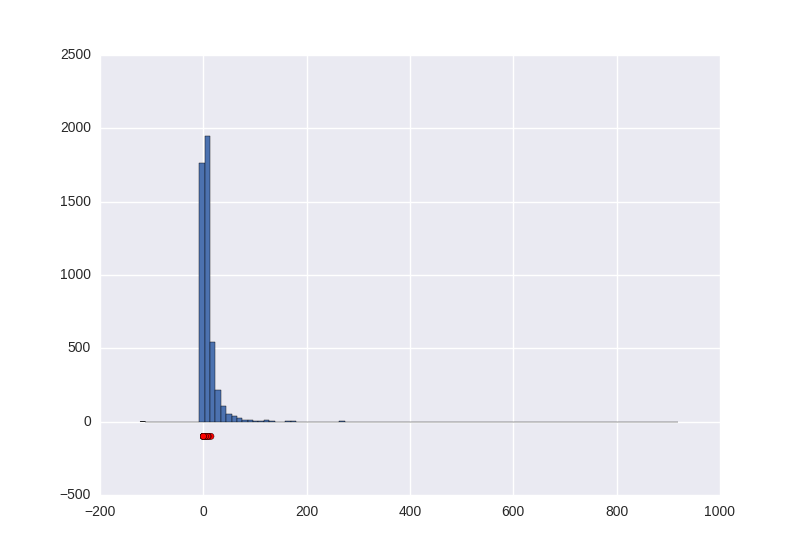
\includegraphics[width=\linewidth]{r20.png}
    \caption{Acquisitions d'immobilisations corporelles / Valeur ajoutée}
  \end{subfigure}
\caption{Diagrammes de distribution}
\end{figure}

\section{Graphiques de dispersion}
Lors de la sélection de notre échantillon d'entreprises saines, nous avons utilise les ratios \emph{marge nette sur ventes, valeur ajoutée par personne, Rentabilité nette des capitaux propres après impôts, Rentabilité nette de l’actif total avant impôts et charges de dettes, Liquidité au sens strict} et \emph{Capitaux propres / Ensemble des moyens d’action}. Nous avons basé cette sélection à l'aide des graphiques de dispersion (au total 420) et d'un calcul de toutes les intersections utilisant spark. La famille retenue est d'une taille comparable à celle des entreprises en faillite (24). Nous présentons ici quelques graphiques croisées des les ratios cités.
\begin{figure}
\captionsetup[subfigure]{labelformat=empty}
\centering
  \begin{subfigure}{.45\textwidth}
    \centering
    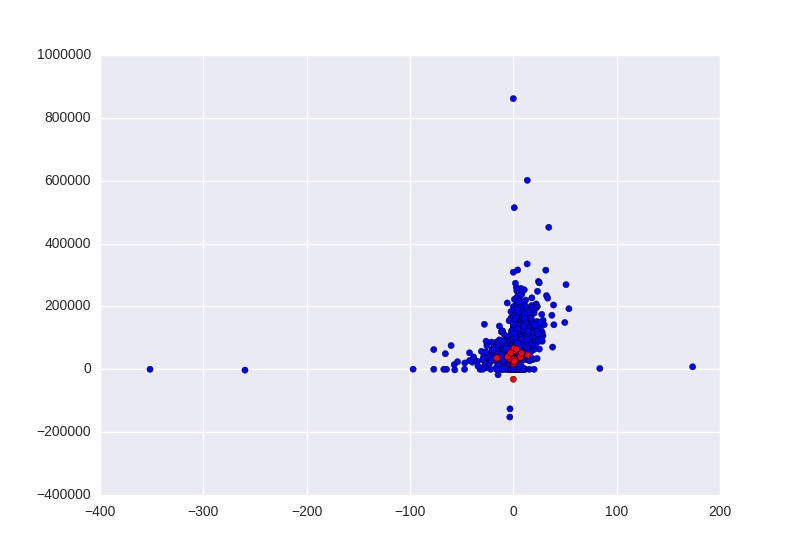
\includegraphics[width=\linewidth]{cr2xr4.png}
    \caption{Marge nette sur ventes et Valeur ajouté par personne}
  \end{subfigure}  
  \begin{subfigure}{.45\textwidth}
    \centering
    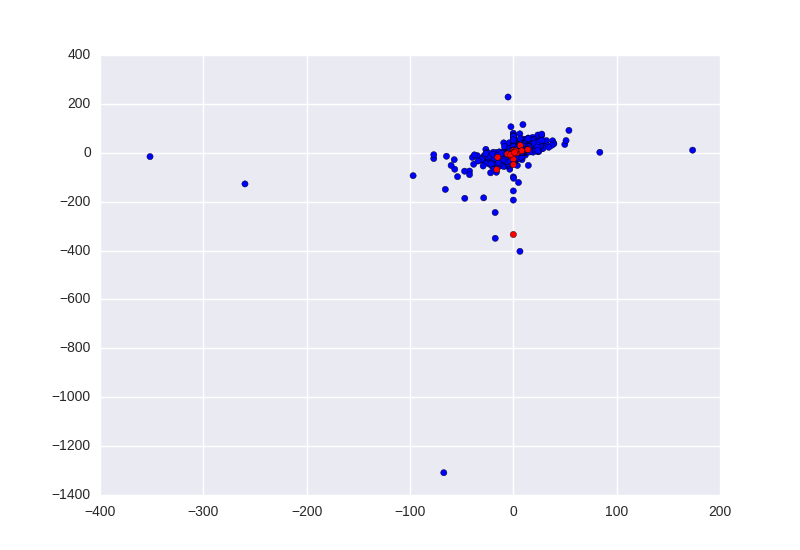
\includegraphics[width=\linewidth]{cr2xr12.png}
    \caption{Marge  sur ventes et Rentabilité nette de l’actif total avant impôts sur charges des dettes}
  \end{subfigure}
  \begin{subfigure}{.45\textwidth}
    \centering
    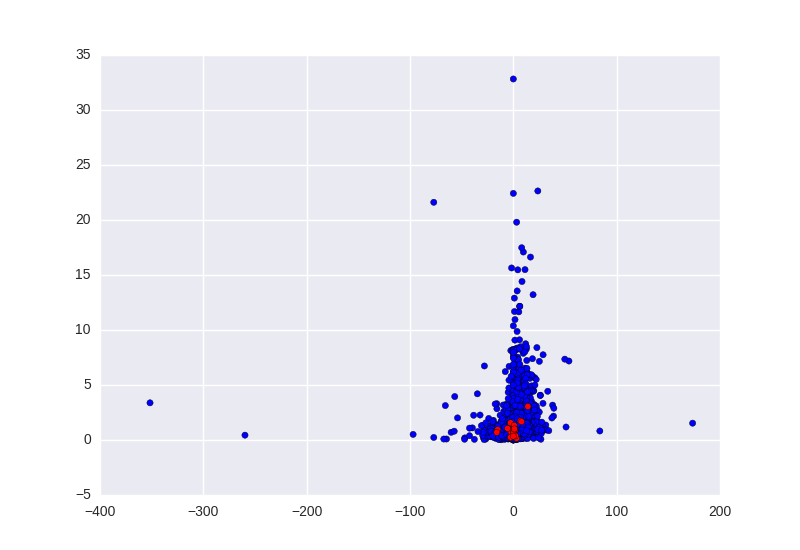
\includegraphics[width=\linewidth]{cr2xr14.png}
    \caption{Marge nette sur ventes et Liquidité au sens strict}
  \end{subfigure}
  \begin{subfigure}{.45\textwidth}
    \centering
    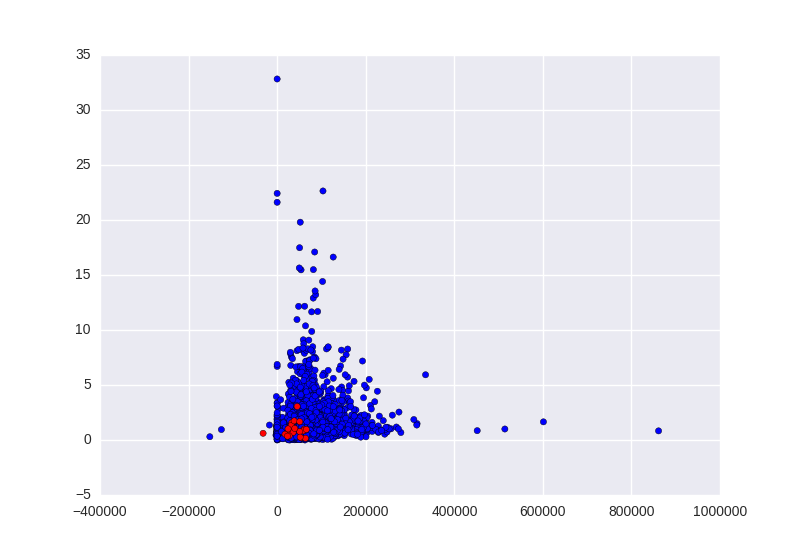
\includegraphics[width=\linewidth]{cr4xr14.png}
    \caption{Valeur ajouté par personne et Liquidité au sens strict}
  \end{subfigure}
  \begin{subfigure}{.45\textwidth}
    \centering
    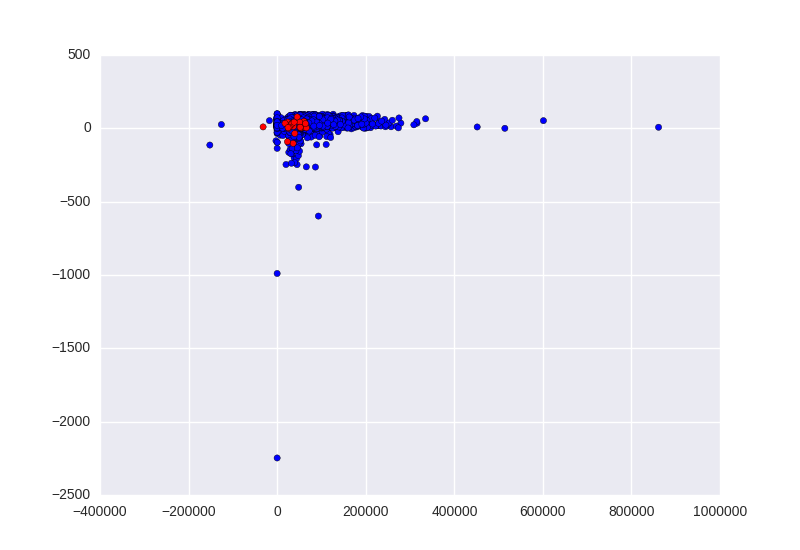
\includegraphics[width=\linewidth]{cr4xr19.png}
    \caption{ Valeur ajouté par personne et Capitaux propres / Ensemble des moyens d’action}
  \end{subfigure}
  \begin{subfigure}{.45\textwidth}
    \centering
    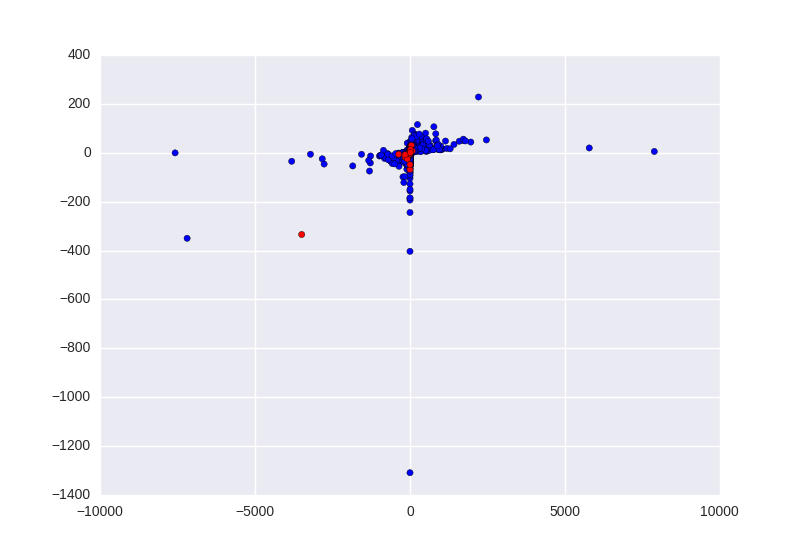
\includegraphics[width=\linewidth]{cr9xr12.png}
    \caption{Rentabilité nette des capitaux propres après impôts et Rentabilité nette de l’actif total avant impôts sur charges des dettes}
  \end{subfigure}
  \begin{subfigure}{.40\textwidth}
    \centering
    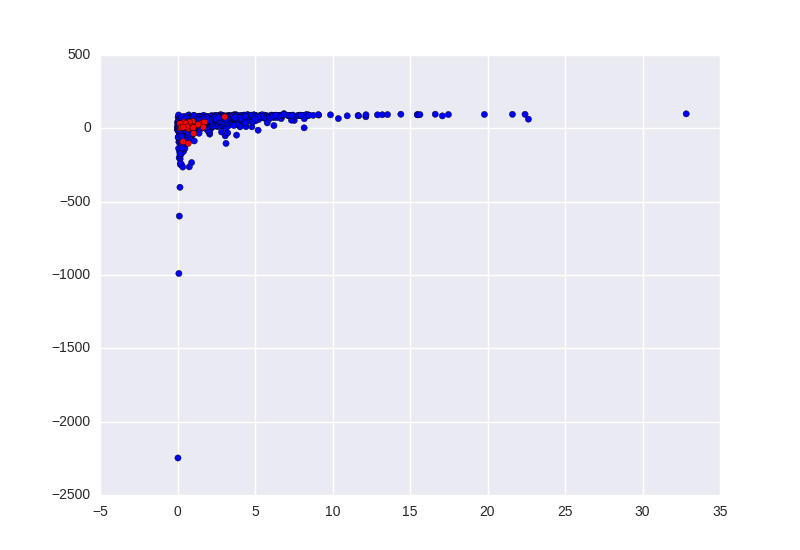
\includegraphics[width=\linewidth]{cr14xr19.png}
    \caption{Liquidité au sens strict et Capitaux propres / Ensemble des moyens d’action}
  \end{subfigure}
\caption{Diagrammes de dispersion}
\end{figure}

\end{appendices}

\twocolumn
\begin{thebibliography}{99} 
\bibitem{Altman}
E. Altman
\newblock Predicting Financial Distress of Companies: revisiting the Z-Score and Zeta Models.
\newblock {\em  New York University}

\bibitem{Bishop}
C. M. Bishop.
\newblock Pattern Recognition and Machine Learning
\newblock {\em Springer}

\bibitem{HTF}
T. Hastie, R. Tibshirani, J. Friedman
\newblock The Elements of Statistical Learning
\newblock {\em Springer}

\bibitem{ross}
S. M. Ross
\newblock Introduction to Probability Models
\newblock {\em Academc Press}

\bibitem{Thibierge}
C. Thibierge
\newblock Analyse Financière
\newblock {\em Vuibert}

\bibitem{wass}
L. Wasserman
\newblock All of Statistics
\newblock {\em Springer}
\end{thebibliography}
%----------------------------------------------------------------------------------------

\end{document}
